Most people have an intuition about what a substance is. A substance is just \textit{something}, like water, wood, butter or glass. A metal is a substance. The blood in your body is a substance. All of these are made up of atoms that form molecules in ways giving them very different properties. We know that a substance can exist in different phases, for example plasma, solid, liquid and gas \cite{ravndal2008statmech}, in which the same substance can behave very differently. Liquids and gases are often called fluids because they share the property that they do not have a fixed shape and are often easily deformed. The theory that describes how fluids behave is called fluid mechanics.

We start this chapter with section \ref{sec:continuum} where we discuss the concept of continuum. This leads to the Euler equations and the Navier-Stokes equations in section \ref{sec:theory_of_fluids_euler_navier}. These equations can be used to study the behavior of fluids in motion relative to the material confining the fluid - fluid flow. We then introduce the concept of porous media, a solid material with parts of its volume - the pore space - available for fluids. Fluids can flow through such a material, and the equation describing the flow rate as a result of some pressure gradient is called Darcy's law. One of the parameters in Darcy's law is called permeability. This quantity is discussed in section \ref{sec:permeability}.

Pore space with channels at the nanometer scale introduces a distinction between what we call macroflows and microflows. This leads to what is called the breakdown of continuum, which is addressed in section \ref{sec:continuum_breakdown}. The Knudsen number is discussed in section \ref{sec:knudsen_number}. It is used to quantify whether or not continuum models can be used, in addition of measuring the importance of slip velocity which has major consequences for the permeability. This is discussed in section \ref{sec:slip_length}. We then discuss particle models - which are not based on the assumption of continuum - in section \ref{sec:theory_of_fluids_atomic_models}. The last two sections are concerned with corrections of the permeability. These are called Klinkenberg correction and Knudsen correction, and use different models for slip velocity to predict the increase in permeability.

\section{The continuum}
\label{sec:continuum}
In reality, we know that a fluid is composed of an enormous number of atoms which are separated by mostly empty space. The atoms interact through quantum mechanics that allows molecules to form. Even though this is the true nature (well, every physicist should be careful to say that something really is the \textit{true nature}) of the fluid, it turns out that we can describe it as a continuum, that is, we assume that the mass is continuously distributed in the total volume of the fluid. This also means that macroscopic quantities like temperature, density, energy and the fluid velocity are well defined in \textit{every} point in space. This is great, continuum mathematics is so much easier to work with than discrete mathematics. Calculus tells us that well behaved functions (as we prefer to work with) can both be integrated and differentiated. They also treat us rather nice, they do what we expect them to do.

In physics we strongly believe in conserved quantities. A fluid in motion will internally (far away from the boundaries in the container) have conserved energy, mass and momentum. This can be formulated beautifully with mathematics, and gives rise to what we today know as the Euler equations and the Navier-Stokes equations.
\section{The Euler equations and the Navier-Stokes equations}
\label{sec:theory_of_fluids_euler_navier}
With the concept of continuum, we think that every point in space has well defined physical properties like temperature, density and momentum. In 1757, Euler published what's called the \textit{Euler equations} by applying conservation of mass, momentum and energy to a small volume element $\dm V$ of a fluid. They form a set of differential equations describing how the fluid velocity $\vec u(\vec r, t)$ field changes in time and space. The conservation laws can be written as
\begin{align}
	\dpart{\rho_m}{t} + \nabla\cdot (\rho_m\vec u) &= 0 \qquad \text{mass}\\
	\dpart{\rho_m \vec u}{t} + \nabla \cdot (\vec u \otimes (\rho_m\vec u)) + \nabla P &= 0\qquad \text{momentum}\\
	\dpart{E}{t} + \nabla\cdot (\vec u(E + P)) &= 0\qquad \text{energy},
\end{align}
where $\rho_m$ is the mass density, $\vec u(\vec r, t)$ is the velocity field, $E(\vec r, t)$ is the total energy per unit volume, $P(\vec r, t)$ is the pressure field and $\otimes$ is the tensor product. These can be combined to one vector equation, but its origin, the connection to conservation laws, is more clear when they are separated like this. In the original paper, Euler only derived the first two equations, but the full set is usually referred to as the Euler equations. They describe the motion of fluids with \textit{negligible viscosity}, which is a decent approximation for many fluids.

Some 80 years later, in the 1840s, Sir George Stokes published the Navier-Stokes equations (NSE) which can be seen as an extension of the Euler equations where effects caused by the viscosity of the fluid are included \cite{batchelor2000introduction}. The Navier-Stokes equations for an incompressible fluid can be written as one vector equation
\begin{align}
	\label{eq:nse}
	\rho_m \frac{D\vec u}{ Dt} = \rho_m \vec F - \nabla p + \mu\nabla^2\vec u + \mu\nabla(\nabla\cdot \vec u)
\end{align}
where $\vec F$ is an external force (i.e. gravity or an electrostatic field), $\mu$ is the viscosity and $D/Dt$ is the material derivative defined as
\begin{align}
	\frac{D}{Dt} = \dpart{}{t} + \vec u\cdot \nabla.
\end{align}
The NSE have quite a few interesting analytically solvable solutions, but for most real systems, the geometry confining the fluid is so complicated that it is usually solved on computers. When solving the NSE, we have to provide boundary conditions to get a unique solution for the system. If we at one end of the container apply some pressure $P_0$, and some other value $P_1$ in the other end, we get a flowing fluid since there acts a net force on the fluid. This defines the pressure difference $\Delta P$. We then also specify the velocity at the boundary which often is the no-slip boundary condition, i.e. that the fluid velocity is zero at the container walls. It turns out that for real fluids, this is not always true. In section \ref{sec:slip_length} we discuss the effects of slip velocity and how this affects the flow properties of the fluid. 
\section{Flow in porous media}
Fluid flow can be defined as fluid in motion relative to its container - the material confining the fluid. A material with parts of its volume available for fluids is called a \textit{porous medium} (see figure \ref{fig:porous_medium}).

\begin{figure}[htb]
\begin{center}
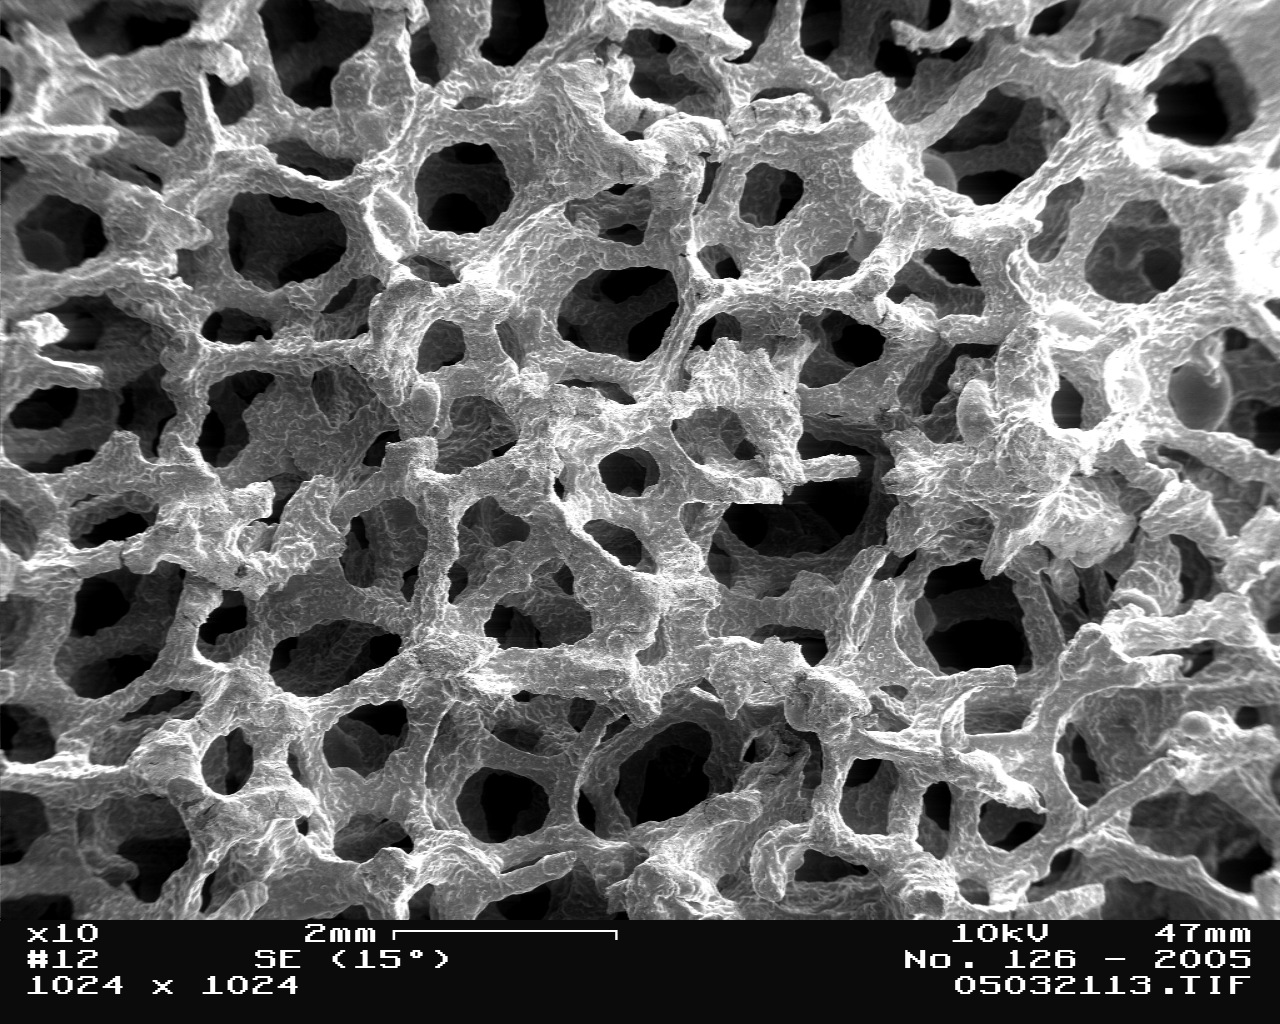
\includegraphics[width=0.8\textwidth, trim=0cm 0cm 0cm 0cm, clip]{figures/metal_foam.png}
\end{center}
\caption{An example of a porous medium. Here we see a metal foam - a solid metal with pore space available for a fluid. A nanoporous medium is a porous medium where the size of the pores are at the nanometer scale. Image from \url{http://en.wikipedia.org/wiki/File:Metal_Foam_in_Scanning_Electron_Microscope,_magnification_10x.GIF}, accessed 28 March, 2014.}
\label{fig:porous_medium}
\end{figure}

We call the larger regions available for fluids \textit{pores} whereas channels connecting these pores are called the \textit{pore network}. All available such space is called the \textit{pore space}. If the porous medium has a total volume $V$, and the pore space takes up a volume $V_p$, we define the \textit{porosity} $\phi$ as
\begin{align}
	\phi = \frac{\text{Pore space volume}}{\text{Total volume}} = \frac{V_p}{V}.
\end{align}
When a fluid flows through the material, the amount that flows through a surface per unit time is called the \textit{volumetric flow rate} and is usually denoted by $Q$. This quantity measures how many cubic meters of fluid we can push through a surface orthogonal to the flow direction per unit time. If we increase the pressure difference, we expect a higher flow rate. This is indeed true. In fact, the volumetric flow rate is proportional to the pressure difference.

\section{Darcy's law}
\label{sec:darcy_law}
When we apply a pressure difference on each side of a material filled with a fluid, the fluid will start to flow in the direction of lower pressure. In 1856, H. Darcy found a linear relation between the pressure difference and the fluid flow rate. This relation is called Darcy's law and tells us what volumetric flow rate $Q$ we can expect from an \textit{incompressible} fluid through a material of length $L$, when we apply a pressure difference $\Delta P$, see figure \ref{fig:darcys_law}. 
\begin{figure}[htb]
\begin{center}
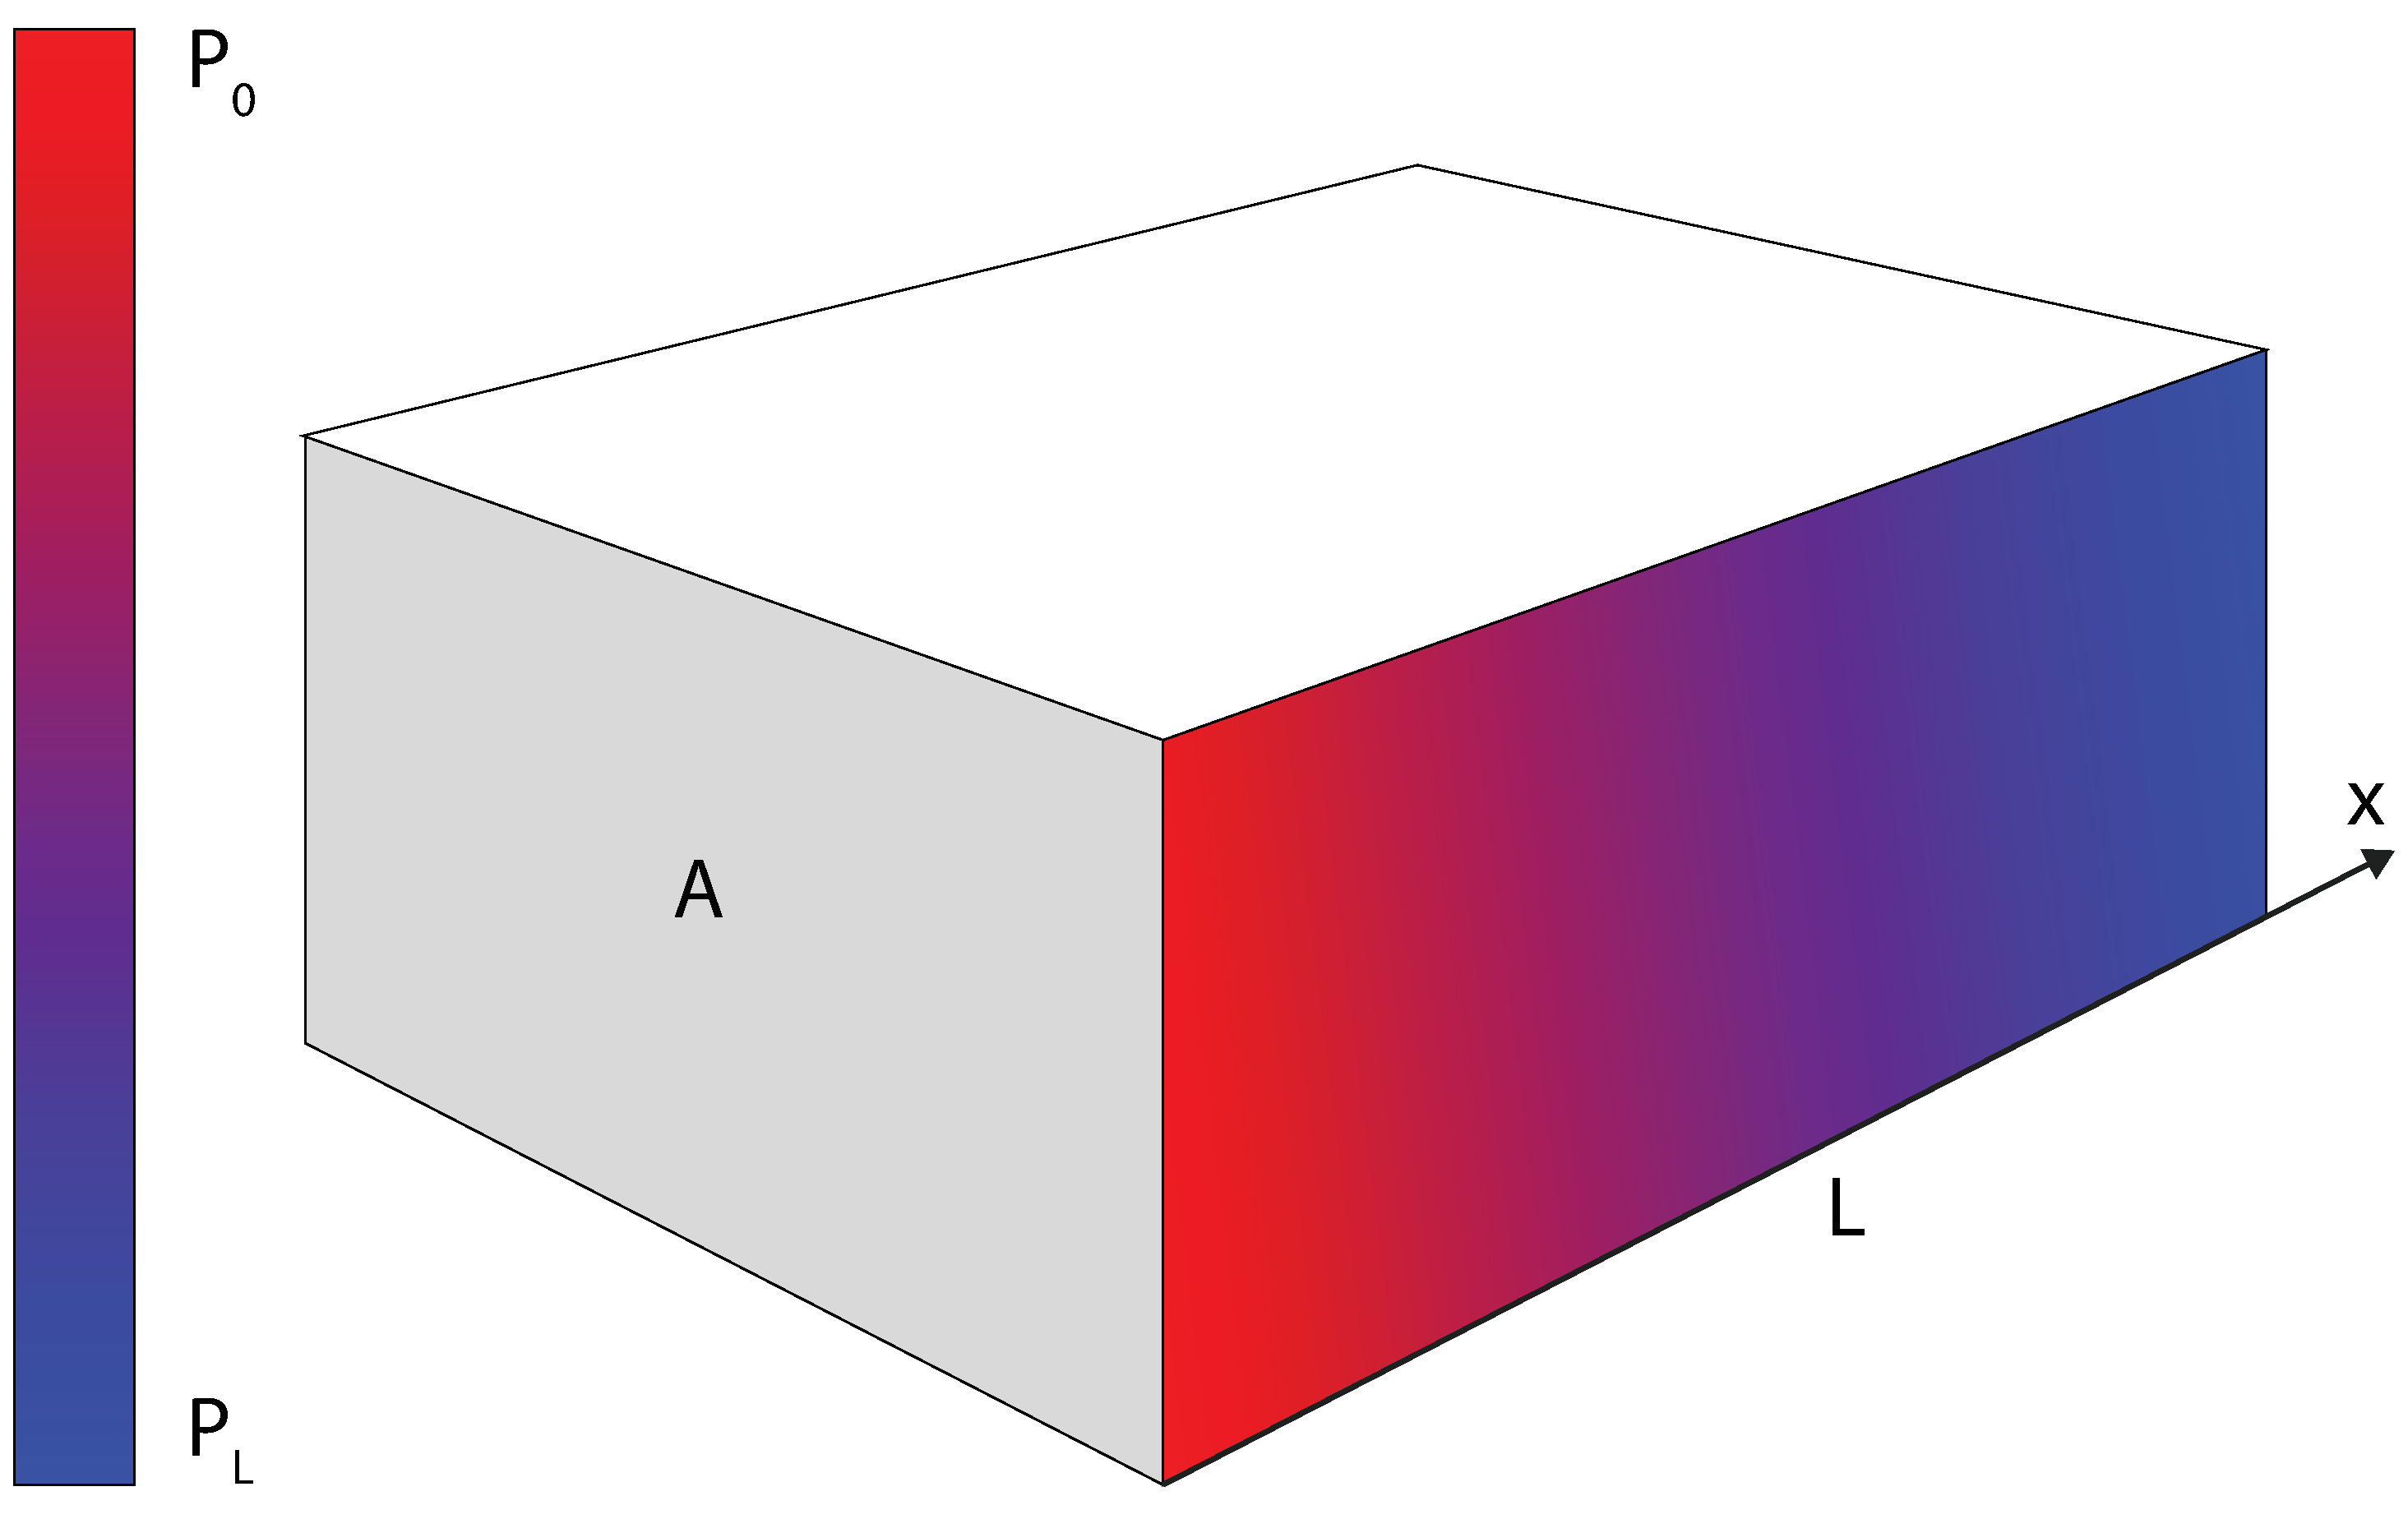
\includegraphics[width=0.75\textwidth, trim=0cm 0cm 0cm 0cm, clip]{kinetic_theory/figures/darcy.eps}
\end{center}
\caption{A box with volume $V=LA$ with fixed pressure values at $x=0$ and $x=L$. The volumetric flow rate $Q$ through a cross sectional area $A$ is given by Darcy's law in equation \eqref{eq:darcy_1}}.
\label{fig:darcys_law}
\end{figure}
The one dimensional version of Darcy's equation is given as 
\begin{align}
\label{eq:darcy_1}
	u = \frac{Q}{A} = \sigma_D\frac{\Delta P}{ L},
\end{align}
where $u$ is the \textit{volumetric flux} (volumetric flow rate per unit area), $\Delta P = P_0 - P_L$ is the pressure difference, $A$ is the cross sectional area; the area of the material orthogonal on the flow direction and $L$ is the length of the material in the flow direction. $\sigma_D$ is the proportionality constant that can be written as
\begin{align}
	\sigma_D = \frac{k}{\mu},
\end{align}
where $\mu$ is the viscosity and $k$ is the permeability.
\section{Permeability}
\label{sec:permeability}
The motivation of introducing the concept permeability is to separate the proportionality constant into two parts; one that depends on the liquid only, the viscosity $\mu$, and the permeability, a material specific constant $k$. This means that we in principle can do an experiment with a liquid with known viscosity, say water, and measure the permeability of some material (Darcy studied a sand filled cylinder in his original experiment). Once you know the permeability, you are able to predict the flow rate through the material for \textit{any} other liquid with a well known viscosity. This is of great importance for i.e. the oil industry where they ideally would like to take a sample of the rock in which the oil or gas is confined, measure the permeability with e.g. air, and then use this to predict the recovery rate.

This is of course not completely true in all circumstances. While Darcy originally found the relation as an empiric equation based on experiments, it can be derived from the Navier-Stokes equations. Darcy's law is only correct if the fluid flow satisfies the no-slip condition.
\section{Macroflows and microflows}
\label{sec:theory_of_fluids_microflows}
In the 1990s H. Bau and J. Zemel performed experiments on microchannel flow in which they found clear deviations from what was expected from the theory\cite{karniadakis2005microflows}. It is useful to introduce the terms \textit{microflows} for flow in geometries where the distance between the channel walls is of order micrometer or smaller, and \textit{macroflows} for larger systems (millimeter and above). Flow at microscales differ from macroscales because of effects that can be classified into four groups
\begin{itemize}
\item non-continuum effects,
\item surface-dominated effects,
\item low Reynolds number effects, and
\item multiscale and multiphysics effects.
\end{itemize}
In this thesis, we focus on the non-continuum effects which are briefly discussed in section \ref{sec:continuum_breakdown}, and the surface-dominated effects as the slip condition described in section \ref{sec:slip_length}. See \cite{karniadakis2005microflows} for details about the effects of low Reynolds number, multiscale and multiphysics. 

\section{The breakdown of continuum}
\label{sec:continuum_breakdown}
As we discussed in section \ref{sec:continuum}, a fundamental assumption in the NSE is that the space is continuous, but we know that in reality, the mass of the fluid is concentrated in the center of the atoms. We often assume that the mass is uniformly distributed in the volume element of which the conservations laws are applied on. This is known as the \textit{continuum hypothesis} and is invalid when the \textit{mean free path} $\lambda$, the average distance a particle moves between collisions, becomes comparable to some characteristic length $L$ in the system, i.e. the diameter of a channel\cite{karniadakis2005microflows}. This is quantified through the \textit{Knudsen number}
\begin{align}
	\text{Kn} = \frac{\lambda}{L}.
\end{align}
From the kinetic theory we can calculate the mean free path (this is done in section \ref{sec:mean_free_path_calculation})
\begin{align}
	\lambda = \frac{m}{\sqrt 2 \pi d^2 \rho_n} = \frac{k_B T}{\sqrt 2 \pi d^2 P},
\end{align}
where $\rho_n$ is the number density and $m$ and $d$ are the mass and diameter of the particles. By using the ideal gas law $P = \rho_n k_BT$, we can replace the density with the pressure $P$ and the temperature $T$. Here $k_B$ is Boltzmann's constant. Molecular Dynamics simulations have shown large fluctuations in temperature and density near the wall in layers a few mean free paths from the surface. Such effects are not reproduced in models based on continuum equations \cite{karniadakis2005microflows}. Another very important effect, as we will discuss in the next subsection, is the non-zero slip velocity of the gas. However, for Knudsen numbers smaller than $10^{-2}$, the continuum hypothesis is valid and we can use continuum equations like the NSE and the Euler equations. It turns out that the Knudsen number is very useful.

\section{Knudsen number}
\label{sec:knudsen_number}
The Knudsen number is the ratio between the mean free path - the average distance a particle moves between colliding with another particle - and a characteristic length in the system. This length could be the radius of a cylinder or the radius of a spherical pore or some other length scale that is representable for the system. In other words, it can be related to how often a particle collides with the surface compared to other particles. A Knudsen number larger than one indicates that a particle travels longer before it collides with another particle than the distance to the surface which means that surface effects are of increasingly importance as the Knudsen number increases.

To get an idea of the length scales where the Knudsen number is about unity, we first need to calculate the mean free path. An oxygen atom in air at room temperature has a mean free path \cite{denny1993air}
\begin{align}
	\label{eq:air_mfp}
	\lambda_{\text{Air}} = \unit{8.0\e{-8}}{\meter},
\end{align}
whereas in water has
\begin{align}
	\label{eq:water_mfp}
	\lambda_{\text{Water}} = \unit{\e{-11}}{\meter}.
\end{align}
This means that air in a nanoporous media with typical pore size about \unit{80}{\nano\meter}, the Knudsen number is of order unity and the continuum hypothesis is invalid. Water in the same system has a Knudsen number approximately $1\e{-4}$ and continuum models should in principle hold. 

\section{Slip velocity}
\label{sec:slip_length}
The usual boundary condition we insert when solving the NSE is the no-slip condition where
\begin{align}
	\vec u(\vec r; t) = 0 \qquad \vec r \in \partial\Omega
\end{align}
where $\partial\Omega$ defines the boundary domain. The history of the no-slip condition was studied by Day\cite{day1990no}, based on the work of Stokes in the 19th century. Stokes compared theoretical results to experiments for pendulums of different kinds and concluded that
\begin{aquote}{Stokes, 1901}
	I shall assume, therefore, as the conditions to be satisfied at the boundaries of the fluid, that the velocity of a fluid particle shall be the same, both in magnitude and direction, as that of the solid particle with which it is in contact. The agreement of the results thus obtained with observation will presently appear to be highly satisfactory.
\end{aquote}
In Day's detailed study of the no-slip condition, he says
\begin{aquote}{Day, 1990}
	Looking back, it appears that the acceptance of a more general no-slip condition was prolonged because of experimental shortcomings, not because of a lack of the \'appropriate\' theoretical solutions to fluid flow problems.
\end{aquote}
In other words, the theoretical framework that existed already in the time of Stokes were complete enough to include both slip and no-slip solutions. In fact, Maxwell predicted slip velocity in a paper already in 1867\cite{maxwell1879stresses}, but the experiments the next 50 years seemed to more or less confirm the no-slip condition.\\
That a fluid has a slip velocity is rather obvious when reading Klinkenberg's nice argument
\begin{aquote}{L.J. Klinkenberg, 1941}
Consider a layer adjacent to the wall which is thinner than the mean free path $\lambda$ of the gas molecules, so that practically a molecule does not collide with other molecules present in this layer. At a given moment half of the gas molecules in this layer will have a component of velocity moving towards the wall; the other half in the opposite direction. The molecules moving towards the wall have had their last collision somewhere in the flowing mass, and, therefore, will have an average velocity component in the direction of flow different from zero. A part of this average velocity component will be lost in colliding with the wall. Even if the molecules lose it entirely, then still the average velocity component in the direction of flow of all the molecules contained in the layer will amount to half of the average velocity component of the molecules moving towards the wall. The gas in the layer, therefore, will have a finite rate of flow.
\end{aquote}
It is convenient to introduce the concept of \textit{slip length} $l_s$ to be able to quantify the slip velocity. Slip length is defined as the distance into the wall we would have to extrapolate a velocity profile for it to reach zero value, see figure \ref{fig:slip_length}.
\begin{figure}[h!]
\begin{center}
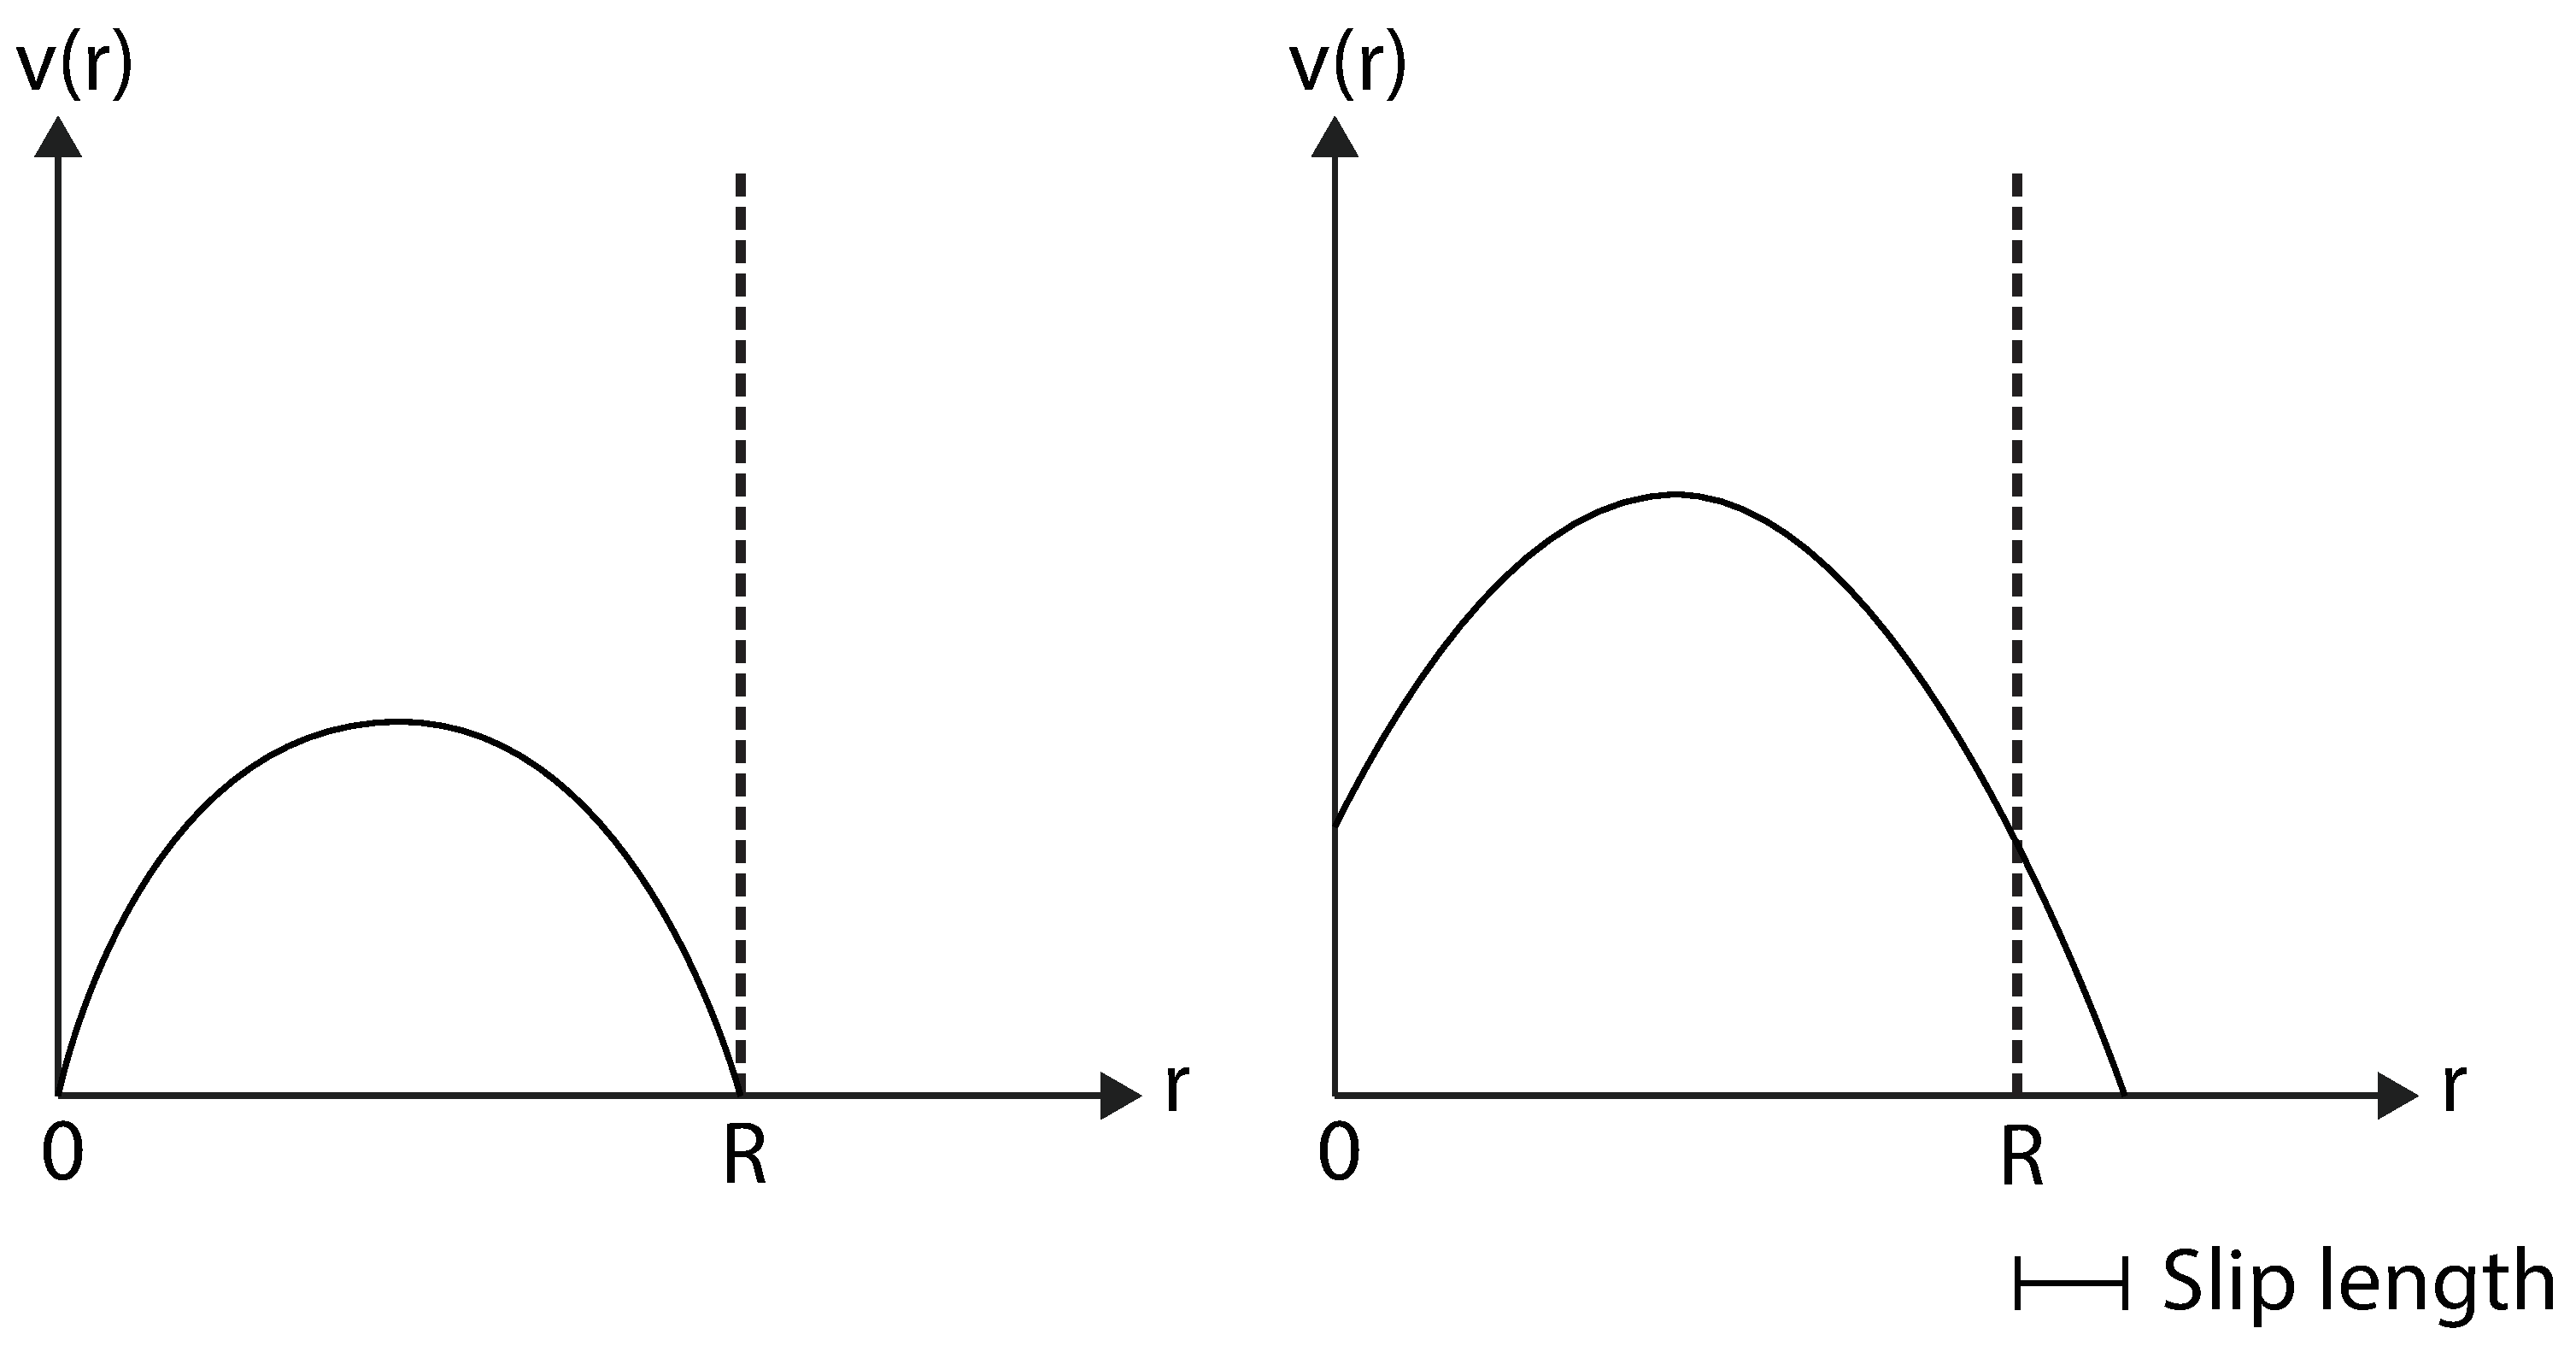
\includegraphics[width=0.8\textwidth, trim=0cm 0cm 0cm 0cm, clip]{DSMC/figures/slip_length.eps}
\end{center}
\caption{Slip length is the distance into the wall we would have to extrapolate a velocity profile for it to reach zero value. We have the no-slip condition on the left, where the slip length is zero whereas we have a non-zero slip length on the right.}
\label{fig:slip_length}
\end{figure}
Maxwell theory predicts the following relation between the slip length and the mean free path
\begin{align}
	\label{eq:noslip_sliplength}
	l_s = \alpha \lambda,
\end{align}
where $\alpha\approx 1.15$ is the slip coefficient \cite{morris1992slip}. The effects of slip velocity become more apparent when the channel diameter is of the same order as the mean free path. By introducing the dimensionless slip length
\begin{align}
	l_s^* = \frac{l_s}{ L} = \alpha \frac{\lambda }{ L} = \alpha \text{Kn},
\end{align}
we see that the ratio of the slip length to the channel diameter is proportional to the Knudsen number. The actual slip velocity (the average velocity of the molecules right next to the wall) can be written as
\begin{align}
	\label{eq:linear_slip_velocity}
	v_{\text{wall}} = \alpha\lambda\frac{\dm v}{\dm n},
\end{align}
where $n$ is the direction normal on the wall\cite{klinkenberg1941permeability}. We call this a \textit{first order} slip model since it is contains only the first derivative of the velocity. Higher order models exists and give corrections that are important in nanoporous media where the channels that contribute to flow are of nanometer scale.

\section{Particle models}
\label{sec:theory_of_fluids_atomic_models}
For systems where the continuum hypothesis is invalid, we need other models describing the behavior of the particles in our system. The first idea that might pop our minds might be to study the system at the atomic level. The equations of motion and hence the dynamics of a system can in principle be calculated directly from quantum mechanics by solving Schr\"{o}dinger's equation. Since this requires calculating the wave function of every atom with complex atomic interactions, the size of the system needs to be very small with today's computers.

An alternative, popular approach is to use a parameterized potential $U(\vec r^N)$ ($\vec r^N$ being the positions of all atoms), and calculate the forces through the gradient of $U$. Newton's equations of motion is then integrated and the dynamics of the system are determined in a classical, deterministic way where important effects from quantum mechanics are embedded in the potential. This method is called \textit{Molecular Dynamics} and is studied in chapter \ref{chap:md}. Molecular Dynamics is orders of magnitudes faster than models solving Schr\"{o}dinger's equation, but it still needs a detailed description of the dynamics of every atom in the system. For many problems, this information is redundant because what's really important is the statistical properties of the system. 

In statistical mechanics, we don't need the full information about every single atom. We can then develop models using statistical mechanics and save a lot of computation power compared to Molecular Dynamics. One such model is called Direct Simulation Monte Carlo and is studied in chapter \ref{chap:dsmc}. The fundamental equation in this case is the Boltzmann equation, which we derive in section \ref{sec:boltzmann_equation}. In the limit of low Knudsen numbers, these models do of course converge towards the continuum models. It is convenient to classify different flow regimes depending on the Knudsen number.
\section{Flow regimes}
We can divide the entire Knudsen range into different regimes enabling us to get an overview of which equations and models that are valid for which Knudsen numbers. In the low Knudsen number limit, the continuum hypothesis is valid and we can in principle use any of the models we have discussed. The continuum approach is here of course preferable since it more computationally efficient compared to the particle models. At some point (Kn$\geq 0.01$), the no-slip boundary condition is invalid and we need to incorporate this into the models solving the NSE in order to get accurate solutions. Here starts the slip regime. When the Knudsen number approaches 0.1, we start to see transitional flow where the flow is laminar near the edges and turbulent in the middle of the material, before we at Knudsen numbers larger than 10 have free molecular flow where the particles almost never interact with each other. This is illustrated in figure \ref{fig:flow_regimes} where we have included the regions where different equations are valid.
\begin{figure}[h!]
\begin{center}
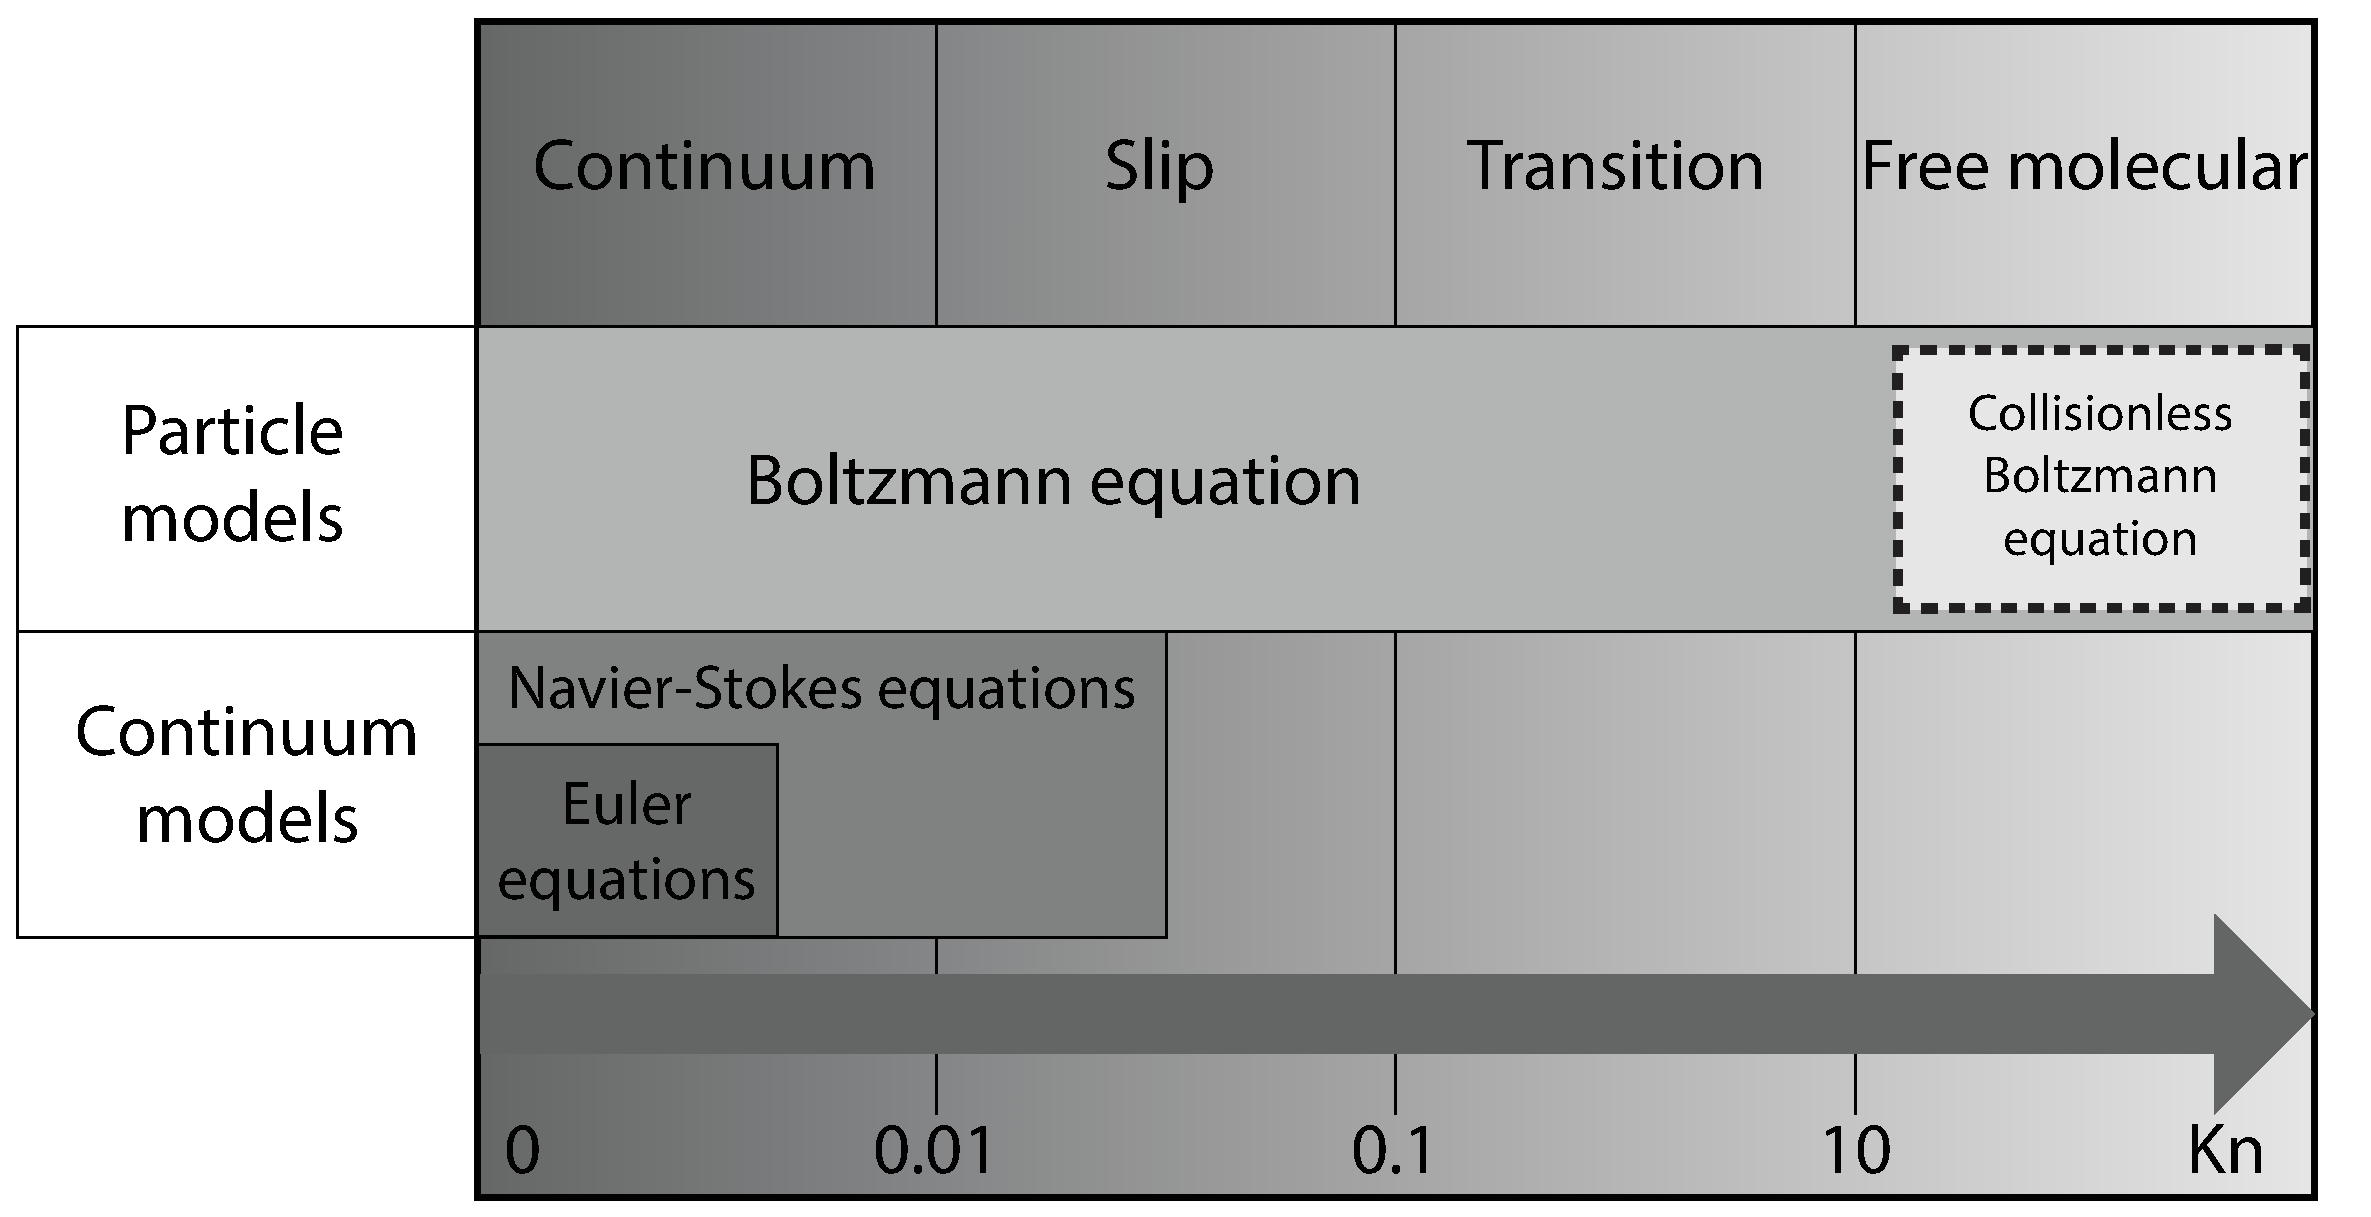
\includegraphics[width=0.8\textwidth, trim=0cm 0cm 0cm 0cm, clip]{figures/flowregimes.eps}
\end{center}
\caption{The four flow regimes covering the important regions in the Knudsen number range where different flow types appear. In the low Knudsen number limit, the fluid can be assumed to be a continuum and we can use equations like the Euler equation or the NSE. For larger Knudsen numbers, the no-slip boundary condition is invalid and we need a model satisfying slip velocity. We reach the transition flow regime at Kn$\approx 0.1$ where the continuum models do no longer hold, even with slip boundary conditions. In the high Knudsen regime particle collisions are so rare that it is classified as free molecular flow. In this range, the collisionless Boltzmann equation is valid (see section \ref{sec:boltzmann_equation}).}
\label{fig:flow_regimes}
\end{figure}